% Chapter 2

\chapter{Problem Definition} % Main chapter title

\label{Chapter2} % For referencing the chapter elsewhere, use \ref{Chapter1} 

\lhead{Chapter 2. \emph{Problem Definition}} % This is for the header on each page - perhaps a shortened title

%----------------------------------------------------------------------------------------
This Thesis addresses the problem of creating a system that allows a human-interactive robot to actively want to learn about novel stumuli presented to it, expanding its knowledge base. Thus, this Thesis deals with the problem of giving a machine the ability of being curious.

Novel stimuli are defined as “different from anything known before; new, interesting and often seeming slightly strange” \cite{Pimentel2014}. We have to identify three aspects of the data; \emph{new}, as not seen anytime before, \emph{interesting}, and \emph{strange}. 

\textbf{New} means that the data entry has not been presented to the system any time before. This aspect will be a characteristic of the data entry itself. \label{new}

\textbf{Strange} data entries are those that do not conform with the base of knowledge, it will be opposite to \emph{known data}. Whereas the aspec \emph{new} refers to the data themselves, \emph{strange} is a prediction made by the model about the data, this prediction is further explained in Section \ref{2.1}. 
Imagine a user poses in front of the camera, every time the user moves and the system records a pose, it will be new. However, the system may classify this new pose as \emph{strange} or \emph{known}, and this is a prediction made by the system, and is subject to the systems performance and accuracy. \label{strange}. The opposite, \emph{known data}, according to the system, is similar to the entries formed by the base of knowledge.

\textbf{Interesting} can be defined as relevant to understand how the system works \cite{Chandola2009}, it is opposite to \emph{noise} An interesting entry has the potential to make our model change or update. The aspect \textbf{interesting} will be directly related to the frequency of appearance of the stimuli. It will also be a prediction made by the model about the data, and  is further explained in Section \ref{2.2}.  For example, similarly to the example proposed in the Introduction of the Thesis in page 1, if the system asked our friend every time he looked to a new girl, our friend would be very annoyed. However, it the system only asked our friend when he looked more than three times to the same girl, probably that girl is interesting to our friend. \label{interesting}. The opposite, \emph{noise} or \emph{noisy data}, is defined as meaningless data.

The following sections expand more these concepts and divide the problem definition in smaller parts:

Section 2.1 Quantifying the strangeness of a stimuli \\
Section 2.2 Quantifying the interest of a stimuli \\
Section 2.3 Learning from novel stimuli \\
Section 2.4 Controlling the curiosity level \\
Section 2.5 Working autonomously and being interactive 
  

\section{Quantifying the strangeness of a stimuli} \label{2.1}

The field of Machine Learning that deals with this task is called \emph{Novelty Detection}. It can be defined as “detecting previously unobserved (emergent, novel) patterns in the data”  \cite{Chandola2009}. \label{novelty}

Typical classification and pattern recognition in Machine Learning deals with two or more classes. The algorithms create a model that is composed of examples from these classes. Then, when presented with a new entry, the algorithms give an estimate of the class this new entry belongs to. 

Novelty detection, instead, tries to detect (or identify) \emph{abnormal data}. That is, data that differs from the data in the training dataset\label{abnormal}. It has become very popular in applications with the need of identifying abnormal behavior. These applications include failure detection in industrial systems, or mass-like structures in mammograms \cite{Pimentel2014}. All this systems have in common that their complexity leads to a limited understanding of a direct identification between a cause and a consequence of what is \emph{normal} and \emph{abnormal}. The problem is that the set of \emph{abnormal} examples is very under-sampled compared with the \emph{normal} set, and also there is a large number of possible \emph{abnormal}  and \emph{normal} modes. In some of the applications there is a high cost of obtaining examples of \emph{abnormal behavior}, for example in industrial damage, to obtain a new abnormal instance one machine has to be broken on purpose, with its associated cost.

This results in typical Machine Learning classification not being suited for these applications. There are not enough examples to create a \emph{normal} class and an \emph{abnormal} class, and there could be multiple unidentified \emph{abnormal} classes.

The approach used by Novelty Detection is a one-class classification. One class, the positive \emph{normal} class must be distinguished from all other possibilities. The positive class must be, then, very well sampled, while the negative \emph{abnormal} classes can be under-sampled. Figure \ref{fig:one} illustrates a 2D representation of a one-class classifier learned from the normal instances, and how anomalies are those instances that are outside the one-class classifier boundary.

\begin{figure}[h]
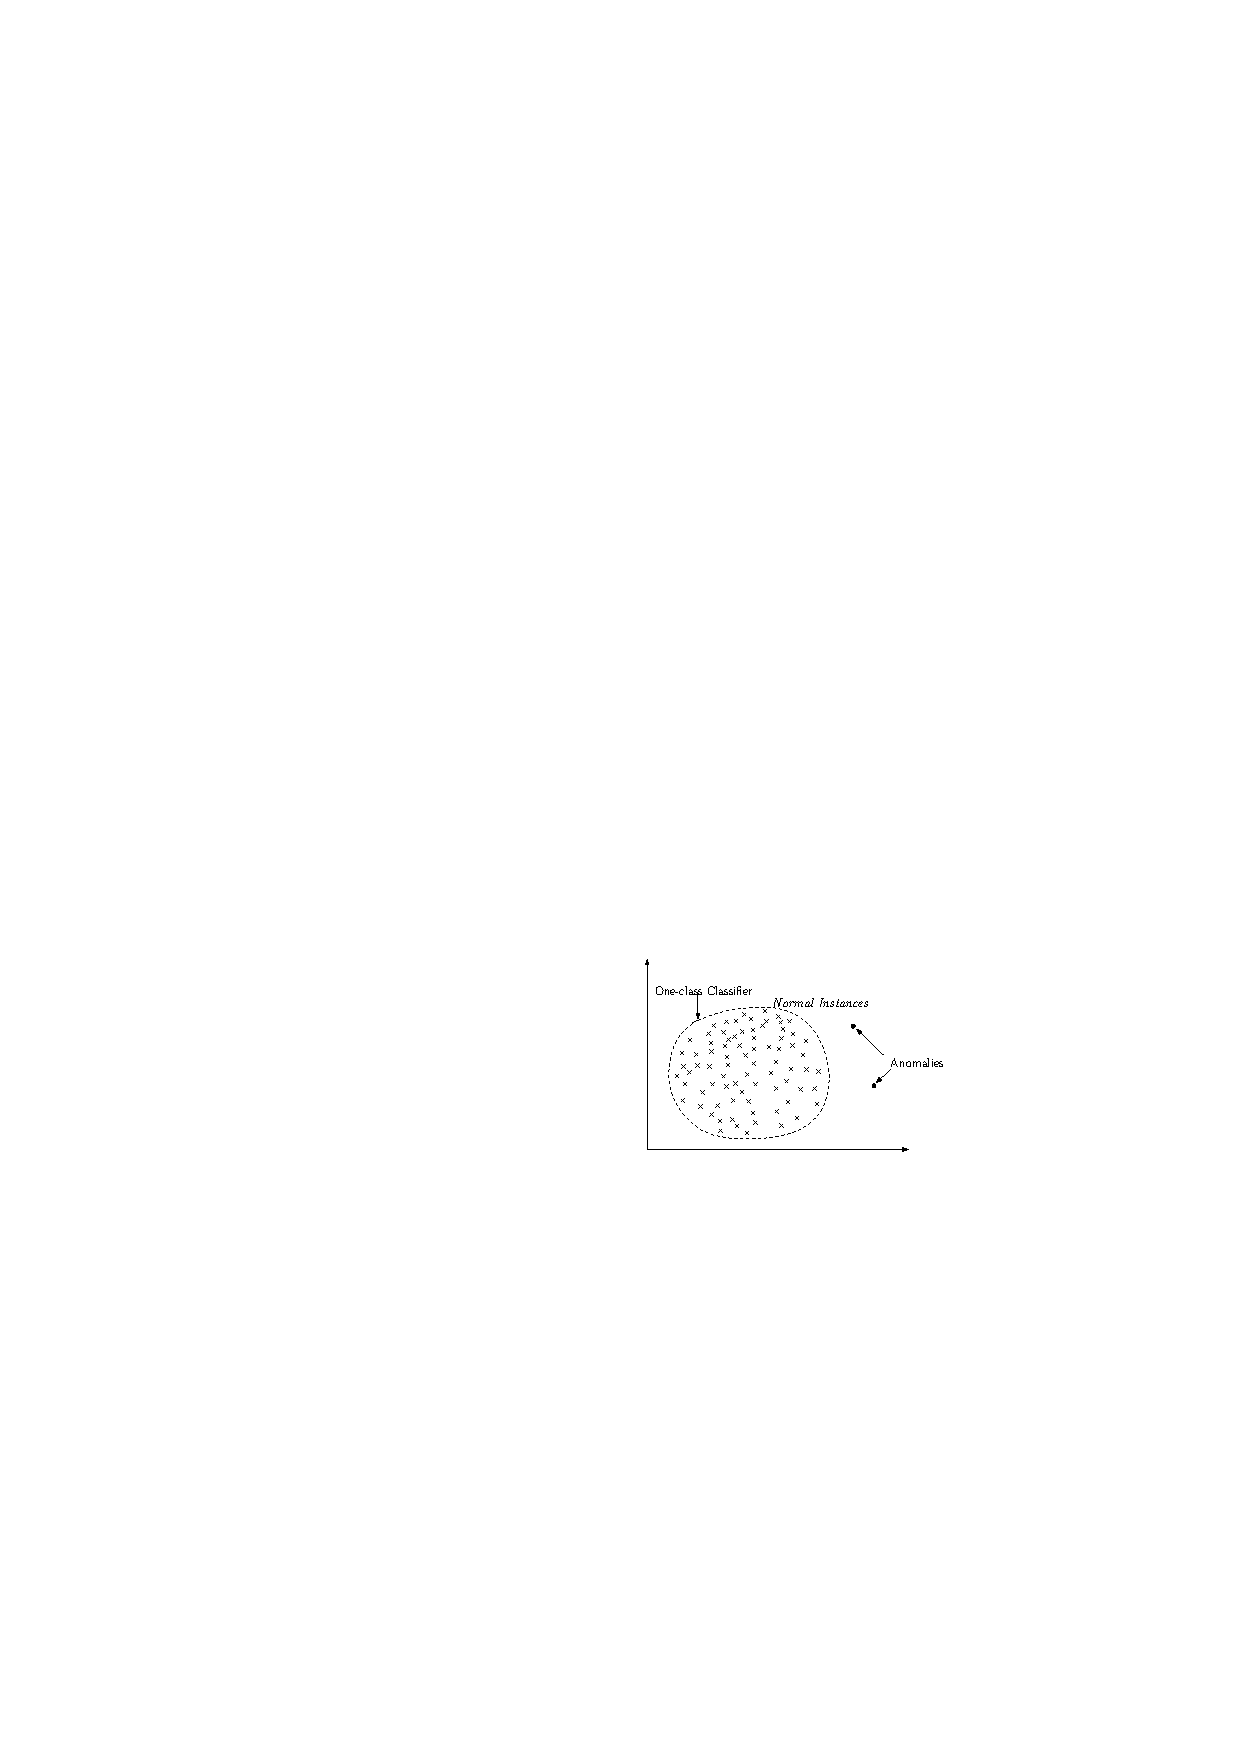
\includegraphics[width=8cm]{Figures/Oneclass}
\centering
\caption[One class Novelty Detection]{One class Novelty Detection. Retrieved from \citeauthor{Chandola2009} \cite{Chandola2009}. \label{fig:one}}
\end{figure}

In the case of the experiment in this Thesis, there are many poses that the user can adopt. It would limit the learning potential of the system to just learn a limited number of the poses and classify the new entries according to them. Instead, the intention of this Thesis if that the system can learn an unlimited number of poses from the user and that the system has the thrive to learn new poses.

The formal approach in Novelty detention is creating a large one-class model of “normality”, formed by as many examples representing normal instances as possible. The new entries are tested against this model of normality, as in Figure \ref{fig:one}, resulting in some sort of \emph{novelty score}. In the case of the figure, \emph{anomalies} would have a high novelty score, while the normal instances inside the boundary would have a low novelty score.

The model of normality is represented as M(\( \theta  \)), where \( \theta  \)
representing the free parameters of the model. This model is used to assign a novelty score, $z(x)$, to test data $x$. A higher novelty score will represent a more \emph{abnormal} instance.

The classification of \emph{normal} or \emph{abnormal} is obtained after comparing the novelty score with a threshold $k$. If:

\begin{equation}
	z(x) \geq  k 
\end{equation}

Then $x$ is classified as \emph{abnormal}. The equation was retreived from \citeauthor{Pimentel2014} \cite{Pimentel2014}.

Different types of models M, methods for setting their parameters \( \theta  \), and methods for determining novelty thresholds $k$ have been proposed in the literature. The classification and further explanation of the Novelty Dectection techniques used will be developed in Section \ref{3.6}.

\label{thresholds}

In \textbf{state-space novelty detection} approaches, the cross-entropy between the normal and the new distributions can be computed. The threshold is set by maximum cross-entropy value computed between the entire training set and each time-series in the training set. Each new entry will be considered normal if its cross-entropy is lower than the values of the entries in the training set \cite{Pimentel2014}.

In \textbf{probabilistic novelty detection} techinques, a novelty threshold may be set yaking into account where the most extreme samples generated from the normal distribution will lie. For example in GMM based algorithms, the threshold is set to be the minimum log likelihood of the training data \cite{Pimentel2014}.

In \textbf{distance based novelty detection} approaches, the distances to the one class centroid for all points in the same scene are computed, and a threshold based on the mean and standard deviation of the distances of the normal instances instances is determined \cite{Pimentel2014}. On other words, if the new point is futher that the average of the training data to the centroid, then its abnormal. 

The methods applied to calculate the threshold in this Thesis are explained in Sections \ref{thres1} and \ref{thres2}.
 
\section{Quantifying the interest of a stimuli} \label{2.2}

The interest of the stimuli is related to classifying the stimuli as interesting or noise. Noise can be defined as a phenomenon in data which is not of interest to the analyst \cite{Chandola2009}. The problem relies in that a noise entry is also an \emph{strange} entry, and will be classified as such. An entry can be detected as strange because it is noise or because it is an novelty, whiwh impies that is interesting by definition. We need to have a filter to separate these two cases, we are only interested learning an entr if it is novel, not if it is noise. We are not interested in adding noise to our model of normality, because that will distrub future novelty detections and may lead to misclassifications.

\begin{figure}[h]
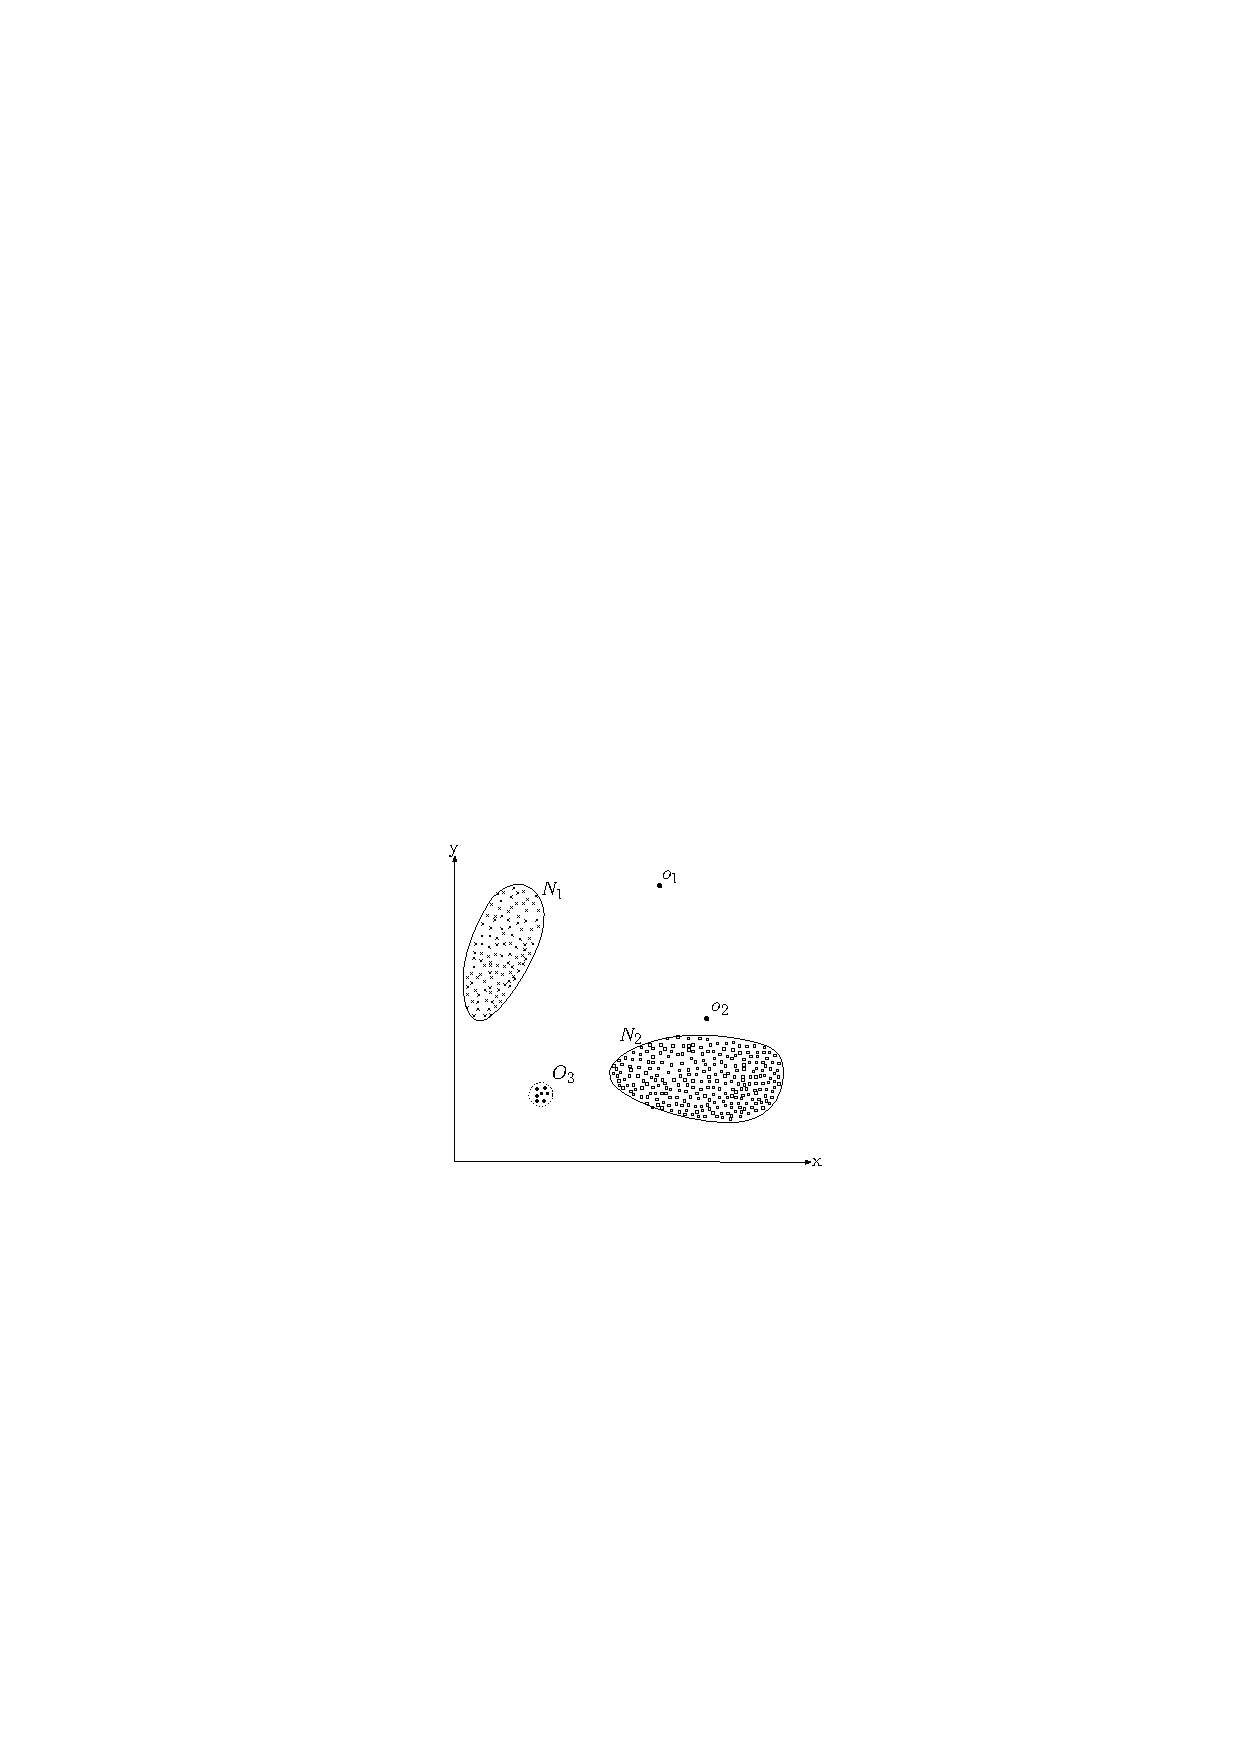
\includegraphics[width=8cm]{Figures/Outliers}
\centering
\caption[Novel and noise entries in 2D.]{Novel and noise entries in 2D. Retrieved from \citeauthor{Chandola2009} \cite{Chandola2009}. \label{fig:out}}
\end{figure}

In Figure \ref{fig:out}, N1 and N2 represent normal data, already added to the model of normality in the one-class classification. 
All instances O1, O2 and O3 will be classified as abnormal, because their novelty score with  be higher than the threshold defined. The difference is that O3 happens more frequently than the other two. This means that we consider O3 more interesting.
The interestingness level may also have a threshold, and the frequency needed for the stimuli to be considered interesting may be changed.

The interest of an stimuli will be directly related to the frequency of appearance of the stimuli with respect to all of the data received by the system up to that point. An application to the “frequent episode discovery problem” in temporal data mining is presented in \cite{frequency}. For a pre-defined confidence level, upper and lower thresholds for the observed frequency of an event can be determined \cite{Pimentel2014}, which can be used to decide whether the event can be considered interesting or noise.

An example of noisy and interesting entries in the experiment this Thesis deals with would be depicted in Figure \ref{fig:noise}.

\begin{figure}[!htb]
\minipage{0.5\textwidth}
  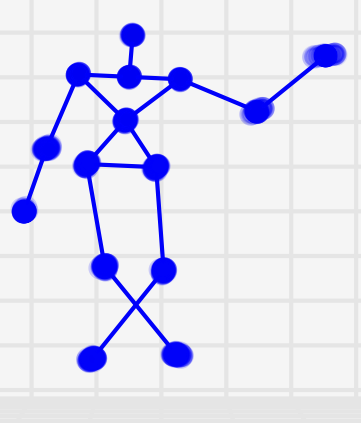
\includegraphics[width=5cm]{Figures/Noise}
  \centering
\endminipage\hfill
\minipage{0.5\textwidth}%
  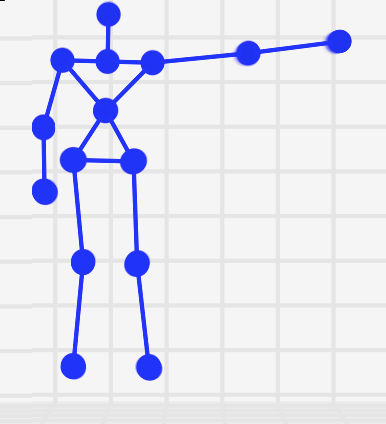
\includegraphics[width=5cm]{Figures/Normal}
  \centering
\endminipage
  \caption{Examples of noisy and insteresting entries in the experiment of pose recognition. \label{fig:noise}}
\end{figure}

Noise in this case would be entries that have been badly recorded by the Kinect, this is further explained in Section \ref{4.2}. In this case, a noisy entry is that where the legs are crossed, because the Kinect could not identify them correctly, and that probably some of the other joints were not recorded properly either. We would expect a noise entry to happen rarely, while the interesting entry will be the type of data we will record frequently.

The idea behind noise detection is that noise is defined to happen very rarely. As mentioned in the previous section, noise is under-sampled with respect to the rest of the data. As can be seen in Figure \ref{fig:out}, interesting events tend to form clusters in the knowledge space, when they are repeated in time in a small area. While noise has a more uniform distribution trougout space, with much less density. There is also a necessity of detecting if a lot of noisy entries are being recorded, because that can mean that there is something wrong with the camera or the processing of the data, and we may need to fix it. So, if a lot of noisy entries are being recorded, then it becomes an interesting event, and thus a novel event. 

As in the previous step, we will need to determine a interest threshold, and compare the interestingness score of the new data with the rest of the entries received. But in this case, the interest threshold is computed from all the entries presented to the system ever, instead of just the model of normality. As we can see in the figure, the interest of the stimuli is determined when taking into account all entries, not just the model of normality. We need to take into account all entries from O3, in Figure \ref{fig:out}, to determine that there is a group of entries that is becoming interesting in that point.  

Thus, the system needs to keep record of two sets of data:

\begin{itemize}

\item A dataset consisting of all the instances every received, including those that have been received but not added to the normal model. This dataset is used to check if the new entries have formed any cluster with previous recorded data, if they are becoming interesting.

\item The normal set, that trains the normality model. Serves to check if the interesting entries are novel or, on the other hand, are something that our system already knows.

\end{itemize}

\section{Learning from novel stimuli}

The last step, after identifying a new stimuli as strange and interesting, is incorporating it to the normal model. This step means adding the entry to the set of data considered as “normal” and recalculating the model for the one-class classification, thus recalculating the threshold values for the novelty score and the frequency of appearance for interesting entries.

This means that when a new stimuli, similar to the previous novel stimuli, is showed to the system, it will now be identified as interesting and normal, as known. 

The approach is based on cumulative learning, because the system accumulates the learned novel poses, expanding continuously its normality model. There are many open challenges related with long-term operation of this system and constraints such as dynamically expandable learning structures and bad learning. We have to deal with the decision of whether to further expand the model when a new perception is misclassified, which may lead to future errors in the learning process. 

This also happens in biological systems, when a baby is taught that an apple is called “pear”, she will identify all future apples as pears, and she will think that she knows the concept when someone mentions a pear to her.

\section{Controlling the curiosity level}

The parameters of the curiosity level of the robot must also be controllable. The programmer is able to choose if the robot is very curious or not.
This is directly related to controlling the novel score threshold and the frequency of appearance for interesting entries. This control will be done by means of a graphic interface where the programmer will be able to tune these parameters.

This aspect is key for the customization of the learning process. Depending on the application, or on the experiment, we may want the system to be very curious or less curious. In our case, we have the objective of not bothering the interacting user too much, but in an application such as video survaillance, probably we want to alert as soon as someone is detected in the camera.

\section{Working autonomously and being interactive}

The system does these active learning tasks autonomously. This means that the retrieval of the data and the computation of the classifications must be fast. The programming will be done using Python and specific Machine Learning libraries, these libraries are referenced in Sections \ref{3.6} and \ref{4.3}.

Altought, was mentioned before, the interaction part is out of the scope of this Thesis, the system needs an interface to communicate to the programmer the outcome of the predictions. Thus, it needs to have a graphic interface to show the results, raise alerts and accept input information from the user.

The only way of going further novelty detection, and deepen in the learning and human-interactive process of the system is asking the user when a novel entry is detected. It is, then, necessary to establish mechanism to display the outcomes from the system to other interactive modules that can actually do the work of interacting with the user. The system needs to provide information about \emph{when} to ask the user.

\begin{flushright}

\end{flushright}
